\documentclass[11pt]{article}
\usepackage{fullpage}
\usepackage{amsthm}
\usepackage{amsmath} 
\usepackage{amssymb}
\usepackage{bm}
\usepackage{graphicx}

\graphicspath{ {./imgs/} }

\setlength{\parindent}{0pt}

\title{Introduction to Machine Learning (CO395)}
\author{Michael Tsang}

\newtheorem{defn}{Definition}
\newtheorem{eg}{Example}
\newtheorem{theo}{Theorem}
\newtheorem{lem}{Lemma}

\begin{document}

\maketitle
\section{Machine Learning}
\textit{The field of machine learning is concerned with the question of how to construct computer programs that automatically improve with experience.}

\subsection{Supervised Learning}
\begin{defn}
Learning an unknown mapping $f(x_i) = y_i$ from training data, given in the form of input  and output pairs $D = \{ (x_i, y_i) \}^N_{i = 1}$.
\end{defn}

\begin{itemize}
  \item $D$ is the \textbf{training set}, $N$ is the number of training examples/samples/data points. 
  \item The $x_i$ are in the \textbf{feature space} $\mathcal{X}$ and the $y_i \in \mathcal{Y}$ are in the \textbf{label space}.
  \item In the simplest setting, each training input $x_i$ is a $D$-dimensional vector of numbers, these are called \textbf{features}, \textbf{attributes}, or \textbf{covariates}.
  \item In general, $x_i$ could be a complex structured object, such as an image or sentence.
\end{itemize}

\subsubsection{Spaces}
\begin{figure}[h]
  \caption{Spaces before the \textit{Deep Learning Era}.}
  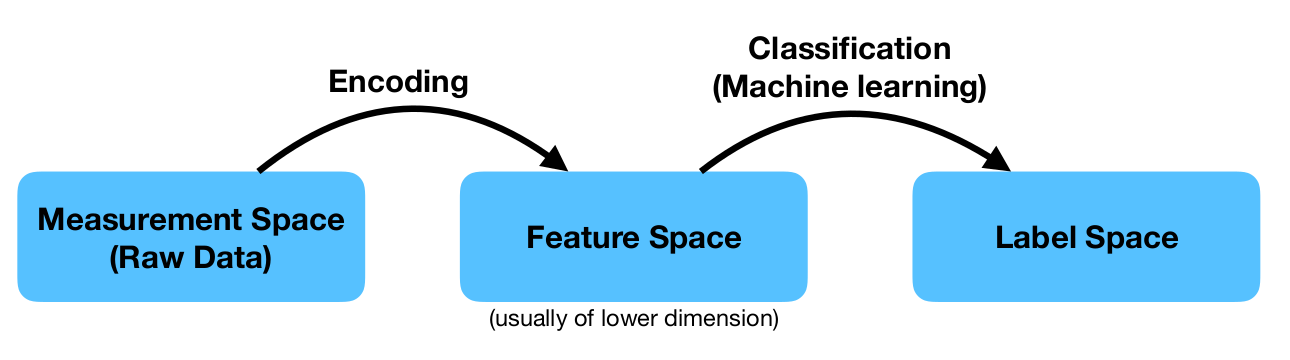
\includegraphics[scale=0.2]{spacesbefore}
  \centering
\end{figure}

\begin{figure}[h]
  \caption{Spaces after the \textit{Deep Learning Era}.}
  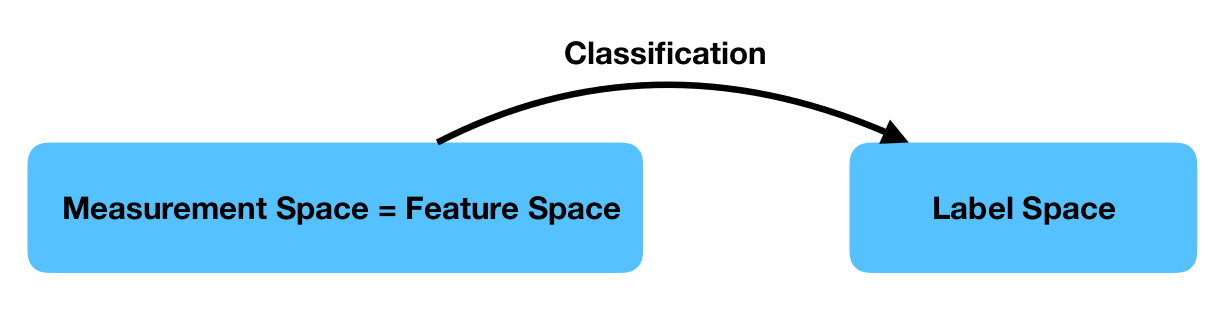
\includegraphics[scale=0.2]{spacesafter}
  \centering
\end{figure}

\subsubsection{Label Space}
There are three main types of \textbf{Label Spaces}:
\begin{itemize}
  \item \textbf{Categorical} (also called class) - $y_i$ is a categorical or nominal variable from some finite set $y_i \in \{1, \ldots, C \}$ (e.g.\ ``Apple'', ``Banana''.).
    The supervised learning task is known as \textbf{classification} or \textbf{pattern recognition}.
  \item \textbf{Real-valued Scalar} - e.g.\ credit score, the task is known as \textbf{regression} or \textbf{function approximation}.
  \item \textbf{Ordinal Regression} - this occurs when the label space has some natural ordering which can be approximated as a regression problem that is subsequently discretised, e.g.\ school grades.
\end{itemize}

\subsection{Unsupervised Learning}
\begin{defn}
Discovering an underlying, hidden, or latent structure within the data $x$.
\end{defn}

The aim is to find a structure that explains the data in a more efficient way.
We can think of this as reducing the amount of bits to store the important features of the data, akin to lossy data compression. \\

This is possible in broadly two ways:
\begin{itemize}
  \item \textbf{Dimensionality reduction} - reducing the dimensions in the data.
  \item \textbf{Clustering} - assigning the data to automatically defined categorical labels.
\end{itemize}

\subsection{Reinforcement Learning}
\begin{defn}
Finding which action to take in order to maximise the received rewards.
\end{defn}

The main differences are:
\begin{itemize}
  \item The best or correct solution is not given to the agent, only a reward signal.
  \item Feedback is delayed.
  \item Time matters, data is sequential.
  \item Agent's decisions affect the subsequent received data.
\end{itemize}

An example of this is in a moving robot.

\subsection{Main Problems in Machine Learning}
\begin{itemize}
  \item \textbf{Classification} - predicting the right label for an unknown sample.
  \item \textbf{Regression} - approximating an unknown function.
  \item \textbf{Clustering} - grouping data in such a way that data points in the same group (cluster) are more similar to each other than to those in other clusters.
  \item \textbf{Dimensionality Reduction} - reducing the dimensionality of the observed data.
  \item \textbf{Density Estimation} - estimating an unobservable underlying probability density function based on observed data.
  \item \textbf{Policy Search} - finding which action an agent should take, depending on its current state, to maximise the received rewards.
\end{itemize}

\section{Instance Based Learning}
We need large amounts of data to make accurate predictions; selecting the right features and representation is crucial.

\subsection{$k$-Nearest Neighbours}
One way of implementing a classifier is to consider the $k$-nearest neighbours in the feature space of the current instance, and \textbf{assign the class in the majority}.

We define the nearest neighbours of a query instance $x_q$ in terms of the Euclidean distance ($L2$-norm):
\[
  d(x_i, x_q) = \sqrt{\sum_g (a_g(x_i) - a_g(x_q))^2}
\]
where the instances $x_i$ belong to the dataset, and all instances are described with a set of $g = [1, \ldots, p]$ features $a_g$.

Alternatively we could use different definitions of distance:
\begin{itemize}
  \item Manhattan ($L1$-norm)
    \[
      d(x_i, x_q) = \sum_g \lvert a_g(x_i) - a_g(x_q) \rvert
    \]
  \item Chebyshev ($L^\infty$-norm)
    \[
      d(x_i, x_q) = \max \lvert a_g(x_i) - a_g(x_q) \rvert
    \]
\end{itemize}

\subsubsection{Choice of $k$}
\begin{itemize}
  \item Small $k$ - Good resolution of class borderlines, but sensitive to noise.
  \item Large $k$ - Bad resolution of class borderlines, but robust to noise.
\end{itemize}

We choose a value of $k$ with a validation dataset.

While the $k$-NN algorithm is powerful, finding the nearest neighbours can be slow if the dataset is large.
Approaches to improve this include: $k$-d trees; Locality-Sensitive hashing with hash tables; or generating prototypes with Learning Vector Quantisation.

\subsection{Distance-Weighted $k$-NN Algorithm}
We assign a weight $w_r$ to each neighbour $x_r$ of the query instance $x_q$ based on the distance $d(x_r, x_q)$: \textbf{nearer neighbours have greater weight}.

Any measure favouring the votes of nearby neighbours works:
\begin{itemize}
  \item Inverse of the distance
    \[
      w_r = \frac{1}{d(x_r, x_q)}
    \]
  \item Gaussian distribution
    \[
      w_r = \frac{1}{\sqrt{2 \pi}} \exp \left(\frac{-d(x_r, x_q)^2}{2}\right)
    \]
\end{itemize}

The value of $k$ is less important as distance examples will have small weight and not greatly affect the classification.

If $k = n$, where $n$ is the total number of instances, the algorithm is a \textbf{global method}.
Otherwise if $k < n$, it is a \textbf{local method}, only takes into account some of the instances. \\

Since classification is based on a weighted combination of all $k$-NN, then the impact of noise is smoothed out - the distance-weighted $k$-NN is \textbf{robust to noisy training data}.

Since the distance is based on all features of each instance, irrelevant features may cause instances that belong in the \textbf{same class to be distant from one another}. \\

To remedy this, we \textbf{weight each feature} differently when calculating the distance.

\subsection{Curse of Dimensionality}
\begin{figure}[h]
  \caption{The relationship between average distance and dimensions.}
  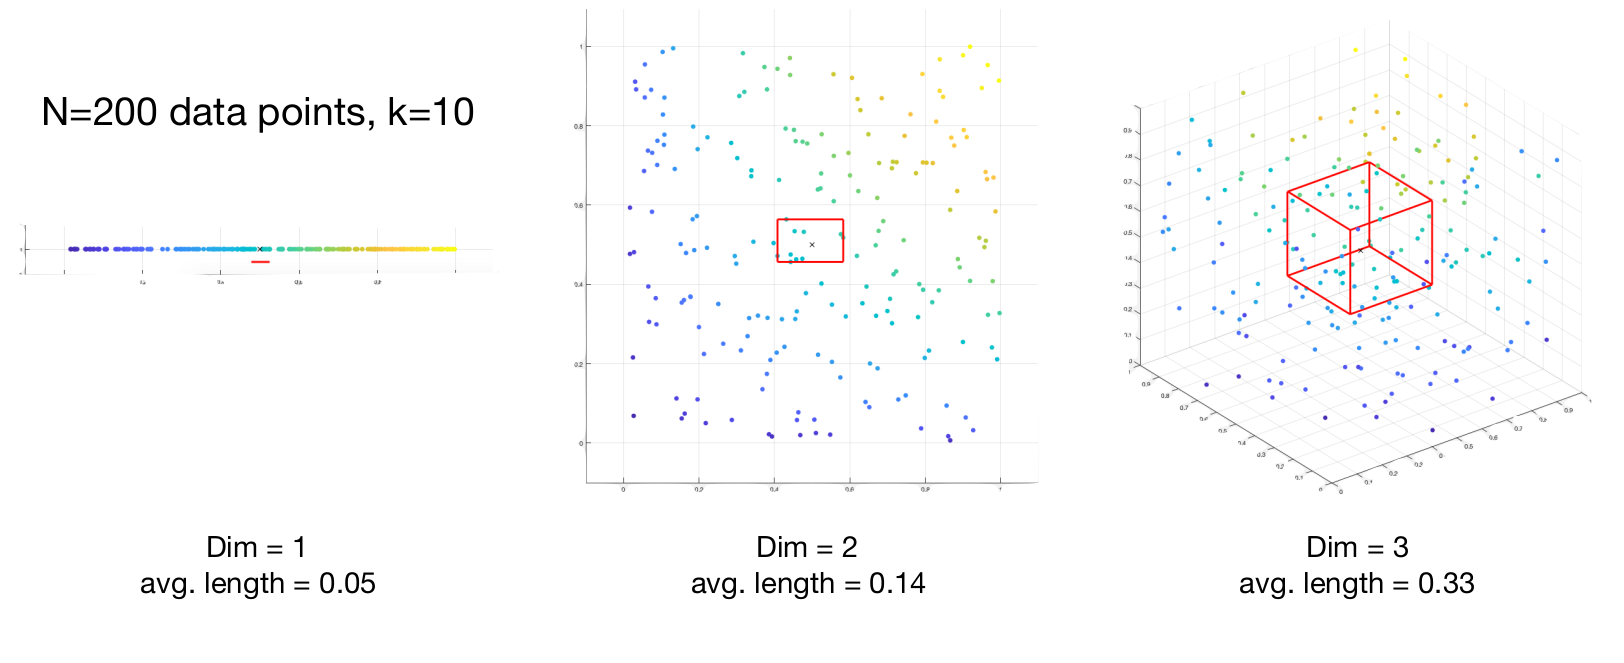
\includegraphics[scale=0.3]{curseofdim}
  \centering
\end{figure}

As the dimensions of the feature space increases, the distance to the nearest neighbours increases.

\subsection{$k$-NN for Regression}
Instead of using the class in the majority, we consider the \textbf{value} in the majority.

In distance-weighted $k$-NN, the prediction of the algorithm is the \textbf{weighted average value} of the $k$-NN.

This is also known as \textit{Locally Weighted Regression}.

\subsection{Lazy Learning}
\begin{defn}
Data is stored, but generalising beyond this is postponed until an explicit request is made.
\end{defn}

\begin{enumerate}
  \item Search the memory for similar instances.
  \item Retrieve the related solutions.
  \item Adapt solutions to the current instance.
  \item Assign estimated solution to the current instance.
\end{enumerate}

An example of this is the $k$-NN algorithm.

\begin{itemize}
  \item A \textbf{different approximation to the target function} is constructed for each query instance.
  \item The collection of \textbf{less complex local approximations} represents a complex target function, where the problem domain could be incomplete.
  \item Large space requirement to store the entire training dataset, with long query time.
  \item Most useful for large datasets with few attributes.
\end{itemize}

\subsection{Eager Learning}
\begin{defn}
  A general, explicit description of the target function is constructed, based on the provided training examples.
\end{defn}

Examples of this are in artifical neural networks and decision trees.

\begin{itemize}
  \item The \textbf{same approximation to the target function} is used, which must be learned based on training examples, and before input queries are observed.
  \item Better memory efficiency, and usually low query time.
  \item Deals better with noise.
  \item Generally unable to provide good local approximations in the target function.
\end{itemize}

\section{Decision Trees}
Decision tree learning is a method for approximating discrete classification functions in a tree-based representation.
A learned decision tree can be represented as a set of if-else rules.

The algorithm is as follows:
\begin{enumerate}
  \item Search for a split point using a statistical test of each attribute to determine how well it classifies the training examples when considered alone.
  \item Split the dataset according to the split point.
  \item Repeat on each of the created subsets.
\end{enumerate}

We choose the split point best on \textbf{information gain}, by quantifying the reduction of the information entropy.

\subsection{Information Entropy}
\begin{defn}
  \textbf{Entropy} is a measure of the uncertainty of a random variable, or the averaged quantity of information required to fully define a random state.
\end{defn}

\[
  H(V) = - \sum_k P(v_k) \log_2 (P(v_k))
\]

For a probability density function $f(x)$, we can define the \textbf{continuous entropy}:
\[
  H(V) = - \int_x f(x) \log_2 (f(x))
\]
$f(x)$ is usually unknown, but can be approximated with density estimation algorithms.

\subsection{Information Gain}
The most informative question in the decision tree maximises the information gain - the difference between the initial entropy and the weighted average entropy of the produce subsets.

\[
  G(q) = H(\text{dataset}) - \left( \frac{\lvert \text{subsetA} \rvert}{\lvert \text{dataset} \rvert} H(\text{subsetA}) + \frac{\lvert \text{subsetB} \rvert}{\lvert \text{dataset} \rvert} H(\text{subsetB}) \right)
\]
where $\lvert \text{dataset} \rvert  = \lvert \text{subsetA} \rvert + \lvert \text{subsetB} \rvert$.

\subsection{Types of Input}
\begin{itemize}
  \item \textbf{Ordered values} (like real-values):
    \begin{enumerate}
      \item For each feature, start by sorting the values of the attribute.
      \item Consider only split points that are between two examples in sorted order that have different classifications.
    \end{enumerate}
  \item \textbf{Symbolic values}:
    \begin{enumerate}
      \item Search for the most informative feature.
      \item Create as many branches as there are different values for this feature.
    \end{enumerate}
\end{itemize}

\subsection{Overfitting}
\begin{figure}[htb!]
  \centering
  \caption{ML algorithm with differing amounts of fit to the data.}
  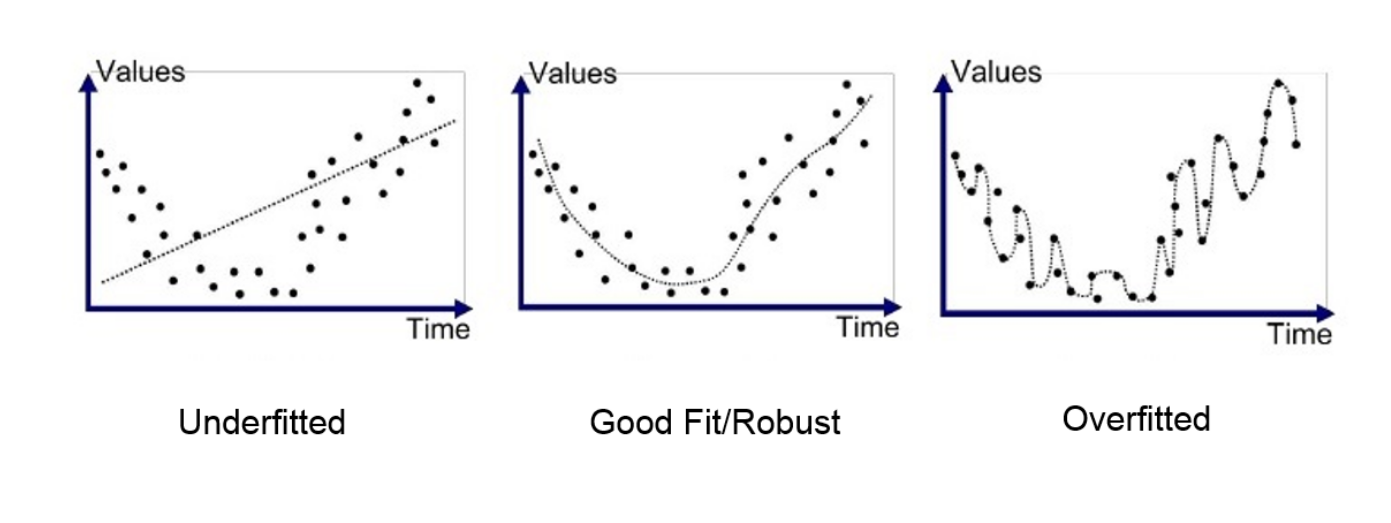
\includegraphics[scale=0.3]{overfitted}
\end{figure}

We can deal with overfitting by splitting the dataset into two parts: \textbf{training} and \textbf{validation}.

We use the training dataset to train the model and the validation dataset to stop the training when performance on the validation test degrades.

\subsubsection{Pruning}
The most common approach with decision trees is \textbf{pruning}.
\begin{enumerate}
  \item Go through all the nodes that are connected to leaves.
  \item Check if the accuracy on the validation dataset would increase if this node is turned into a leaf.
\end{enumerate}
This may need to be done recursively.

\subsection{Regression}
Decision trees can be used for classification and regression, though the former is much more common.
We call a decision tree used for regression a \textbf{regression tree}.

Instead of a single class in each leaf, there is a linear function of some subset of the numerical features.
This requires that the learning algorithm decide when to stop splitting and begin applying linear regression over the features.

\section{Evaluating Hypotheses}
The ultimate goal in machine learning is to create models or algorithms that can generalize to unknown data.

To ensure meaningful evaluation, we use a \textbf{test dataset}.
This should \textbf{not} be used to train the model - it simulates unknown data.

\subsection{Parameter Tuning}
We want to find good parameter values that work with unknown data.

\textbf{Incorrect} approaches:
\begin{itemize}
  \item Try different values on the training dataset, select the best according to the accuracy on the training dataset.
    \begin{itemize}
      \item May not generalize well.
    \end{itemize}
  \item Try different values on the training dataset, select the best according to the accuracy on the test dataset.
    \begin{itemize}
      \item The test dataset is now part of the training process.
      \item Cannot evaluate how the algorithm generalizes to unknown data.
    \end{itemize}
\end{itemize}

\subsubsection{The Correct Approach}
\begin{itemize}
  \item Split dataset into \textbf{training}, \textbf{validation}, and \textbf{test}.
  \item Usually $60\%/20\%/20\%$ split.
  \item Try different values on the training dataset, select the best according to accuracy on the validation dataset, and perform the final evaluation on the test dataset.
  \item Parameter choice takes into account how the model would generalise, and final evaluation considers only unknown data.
\end{itemize}

\subsection{Holdout Method}
\begin{enumerate}
  \item Keep the classifier that leads to maximum performance on the validation set - \textbf{parameter optimization/tuning}.
  \item Parameters are fixed, can choose to use the model trained on the training dataset, or combine the training and validation datasets to train a new model (with the same parameters).
  \item Finally, evaluate on the test dataset.
\end{enumerate}

Once parameters are fixed and we have an estimation for the performance of the model, we retrain it on the \textbf{entire dataset} (including test) as we want the best model.

\subsection{Cross Validation Method}
With a small sample size, a better alternative is to use \textbf{cross validation}.

\begin{enumerate}
  \item Divide the dataset into $k$ (usually $10$) folds.
  \item Use $k - 1$ for training and validation, $1$ for testing:
    \begin{itemize}
      \item Test data between different iterations should never overlap.  
      \item Training/validation and test data in the same iteration should never overlap.
    \end{itemize}
  \item In each iteration, the error on the test set is estimated.
  \item We calculate the average of the $k$ errors: $\frac{1}{N}\sum_{i = 1}{N} e_i$.
\end{enumerate}

\subsubsection{Parameter Tuning}
\begin{enumerate}
  \item Divide the $k-1$ folds into training and validation folds: $k - 2$ for training, $1$ for validation.
  \item Train on the training set, optimize parameters on the validation set, test on the test set.
\end{enumerate}
We can only estimate the test set performance, we evaluate how our implementation generalizes on unknown test sets.

We know nothing about the optimal parameters - we find a different set of optimal parameters in each fold.

Once we know the average accuracy of the model, we use the entire dataset to estimate the optimal set of parameters:
\begin{enumerate}
  \item $k-1$ folds for training, $1$ for validation.
  \item For each parameter, run the $k$ fold cross validation.
  \item Select the parameters that result in the best average performance over all $k$ left out folds.
\end{enumerate}

\subsection{Metrics}
\subsubsection{Confusion Matrix}
\begin{center}
  \begin{tabular}{c c c}
    & Class 1 Predicted & Class 2 Predicted \\
    Class 1 Actual & \textbf{TP} & \textbf{FN} \\
    Class 2 Actual & \textbf{FP} & \textbf{TN}
  \end{tabular}
\end{center}
We use the confusion matrix to visualize the performance of an algorithm and to calculate other performance measures.

The table highlights the risk of each prediction - in some cases it may be more important to have low false negatives than low false positives.

\subsubsection{Classification Rate}
\[
  \frac{TP + TN}{TP + TN + FP + FN}
\]
\begin{itemize}
  \item The number of correctly classified examples divided by the total number of examples.
  \item $\text{Classification Error } = 1 - \text{ Classification Rate}$.
  \item The probability of a correct classification.
\end{itemize}

\subsubsection{Recall}
\[
  \frac{TP}{TP + FN}
\]
\begin{itemize}
  \item The number of correctly classified positive examples divided by the total number of positive examples.
  \item High recall - class is correctly recognized.
  \item Probability of a positive example being classified as such.
\end{itemize}

\subsubsection{Precision}
\[
  \frac{TP}{TP + FN} 
\]
\begin{itemize}
  \item The number of correctly classified positive examples divided by the total number of predicted positive examples.
  \item High precision - a positively labeled example is positive.
  \item Probability that a positively classified example is positive.
\end{itemize}

\subsubsection{Precision and Recall}
\begin{itemize}
  \item High recall, low precision - most positive examples are correctly recognized but there are a lot of false positives.
  \item Low recall, high precision - lots of missed positive examples, but those predicted as positive are positive.
\end{itemize}

\subsubsection{Unweighted Average Recall}
The mean of the recall of each class.

\subsubsection{F-Measure/Score}
\begin{align*}
  F_\alpha &= (1 + \alpha^2)\frac{\text{Precision } \times \text{ Recall}}{(\alpha^2 \times \text{ Precision}) + \text{ Recall}} \\
  F_1 &= 2\frac{\text{Precision } \times \text{ Recall}}{\text{Precision } + \text{ Recall}}
\end{align*}

\subsection{Imbalanced Test Set}
In a balanced dataset, the number of examples in each class are similar - all measures result in similar performance.

In an imbalanced dataset, the classes are not equally represented:
\begin{itemize}
  \item CR is affected a lot by the majority class.
  \item Precision for minority classes are significantly affected - examples belonging to the majority are misclassified.
  \item UAR can detect that one class is misclassified, but gives no information on false positives.
  \item F1 can be useful, but also affected by the class imbalance problem.
\end{itemize}

It is important to look at the confusion matrix.

\subsubsection{Solutions to the Imbalance Problem}
\begin{itemize}
  \item We can divide each value in the confusion matrix by the total number of examples.
    \begin{itemize}
      \item These would be the results if we had the same number of examples and the performance of the classifier remained the same.
      \item There is no guarantee the performance would remain the same.
    \end{itemize}
  \item Upsample the minority class.
  \item Downsample the majoirty class.
\end{itemize}

\subsection{Overfitting}
\begin{defn}
  \textbf{Overfitting} gives good performance on the training data but poor generalization to other data.
\end{defn}

\begin{defn}
  \textbf{Underfitting} gives poor performance on the training data and poor generalization to other data.
\end{defn}

Overfitting could occur when:
\begin{itemize}
  \item Learning performed for too long.
  \item Examples in the training set not representative of all possible situations.
  \item Model too complex.
\end{itemize}

We can fight overfitting by:
\begin{itemize}
  \item Stopping training earlier - use validation set to know when.
  \item Get more data.
  \item Use the right level of complexity - validation set.
\end{itemize}

\subsection{Comparing Algorithms}
\subsubsection{Error}
\begin{defn}
  The \textbf{true error} of the model $h$ is the probability that it will misclassify a randomly drawn example $x$ from distribution $D$:
  \[
    \text{error}_D(h) = P(f(x) \neq h(x)) 
  \]
\end{defn}

\begin{defn}
  The \textbf{sample error} of the model $h$ based on a data sample $S$ is:
  \[
    \text{error}_S(h) = \frac{1}{N} \sum_{x \in S} \delta(f(x), h(x))
  \]
  where:
  \begin{align*}
    N &= \text{ number of samples} \\
    \delta(f(x), h(x)) &= 1 \text{ if } f(x) \neq h(x) \\
    \delta(f(x), h(x)) &= 0 \text{ if } f(x) = h(x)
  \end{align*}
\end{defn}

We want to know the true error but can only measure the sample error.

\subsubsection{Confidence Interval}
\begin{defn}
  A $N\%$ \textbf{confidence interval} for some parameter $p$ is an interval that is expected with probability $N\%$ to contain $p$.
\end{defn}

Given a sample $S$, we can say with $N\%$ confidence, the true error lies in the interval:
\[
\text{error}_S(h) \pm Z_N \sqrt{\frac{\text{error}_S(h) \times (1 - \text{ error}_S(h))}{n}}
\]

\subsubsection{Comparing Two Algorithms}
We run a statistical test to tell us if there is a difference between two distributions of classification errors, in order to see which is better.

Our tests return a \textbf{p-value}.
We make our \textbf{null hypothesis} the case that there is no performance difference between the two algorithms tested.
If the performance difference is \textbf{statistically significant} ($p < 0.05$), then we reject the null hypothesis.

A higher p-value does not mean the algorithms are similar, only that there is no observable statistical difference.

Other notes:
\begin{itemize}
  \item The evaluation of a model represents what performance can be expected when applying the model on a similar data distribution.
  \item If the model is stochastic, we should replicate the training several times to know the distribution of the performance.
\end{itemize}

\section{Neural Networks}
\begin{figure}[htb!]
  \centering
  \caption{A single neuron.}
  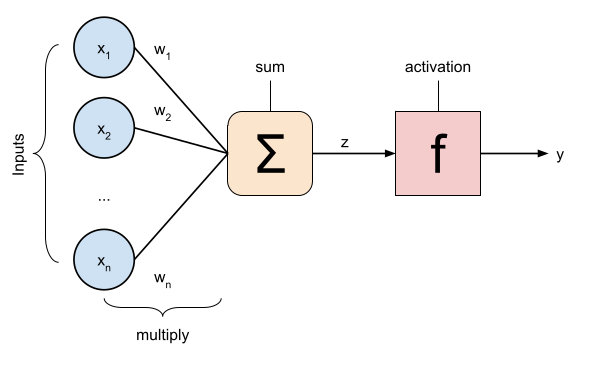
\includegraphics[scale=0.5]{neuron}
\end{figure}

Every \textbf{input} $x_i$ is multiplied by its corresponding \textbf{weight} $w_i$ then summed to get $z$, the \textbf{pre-activation value}, which is then passed to the \textbf{activation function} $f$:
\[
  y = f(z) = f \left( \sum_i w_i x_i \right) = f (w^\intercal x)
\]
In vector form, $w, x \in \mathcal{R}^{n \times 1}$.

We can simplify to a single input:
\[
  y = f(wx) 
\]
which resembles the function of a line $y = wx + b$, without the \textbf{bias}.
If $x' = \begin{pmatrix} x \\ 1 \end{pmatrix}$ and $w = \begin{pmatrix} w_1 \\ w_0 \end{pmatrix}$, then we get $y = w_1 x + w_0$ - the same as having an explicit bias value.

\subsection{Perceptron}
Suppose we have some labelled data $x^{(1)}, x^{(2)}, \dots$ which have some desired outputs $y^{(1)}, y^{(2)}, \dots$.
We are trying to do binary classification, the class is either $0$ or $1$.
We take the activation function to be a \textit{threshold function}:
\[
  h_w(x) = f(w \cdot x) = 1 \text{ if } w \cdot x \geq \theta \text{ else } 0
\]

\begin{defn}
  The \textbf{percepton learning rule} to update the weights in order to learn this classification is:
  \[
    w_i \leftarrow w_i + \alpha(y - h_w(x)) \times x_i
  \]
\end{defn}
The $\alpha$ is the \textbf{learning rate}:
\begin{itemize}
  \item If $y = h_w(x)$, then the weights stay the same.
  \item If $y = 1; h_w(x) = 0$, then the corresponding weight is increased when the $x_i$ is positive, and decreased when it is negative - we want to increase the summation.
  \item If $y = 0; h_w(x) = 1$, then the opposite happens - we want to decrease the summation.
\end{itemize}

A perceptron can learn any \textbf{linearly separable function}, but cannot handle an \textit{XOR} case - we cannot draw two lines to separate the classes.
We need to transform the \textit{XOR} into a linearly separable problem, what if the transformation was learned?

\subsection{Layers}
When we have multiple outputs or want to learn multiple intermediate transformation or features of the input, we need many neurons.
\begin{defn}
  A \textbf{layer} is a collection of neurons that share the same inputs but have different weights.
\end{defn}

We still have the input $x \in \mathcal{R}^{N \times 1}$, but we can collect the weights into a matrix $W \in \mathcal{R}^{N \times M}$, with bias $b \in \mathcal{R}^{M \times 1}$, producing outputs $y \in \mathcal{R}^{M \times 1}$:
\[
  y = f(W^\intercal x + b) 
\]

Every neuron has the same computation but different weights - each neuron creates a learnable linear combination of its inputs passed through a non-linear activation function $f$, the layer now computes $M$ many different transformations of the input.

The scalar activation function is applied element-wise:
\[
  f(\textbf{x}) = 
  f 
  \left( 
    \begin{pmatrix}
      x_1 \\ x_2 \\ \vdots
    \end{pmatrix}
  \right) 
  =
  \begin{pmatrix}
    f(x_1) \\ f(x_2) \\ \vdots
  \end{pmatrix}
\]
There is no requirement to apply the activation within the layer - we can separate activation from the linear transformation:
\begin{align*}
  z &= W^\intercal x + b &
  y &= f(z)
\end{align*}

\begin{defn}
  A \textbf{fully-connected} or \textbf{dense} layer is when every input is connected to every neuron; the number of neurons in these layers is referred to as \textbf{units}.
\end{defn}

\subsection{Feed-Forward Networks}
\begin{figure}[htb!]
  \centering
  \caption{Feed-forward neural network.}
  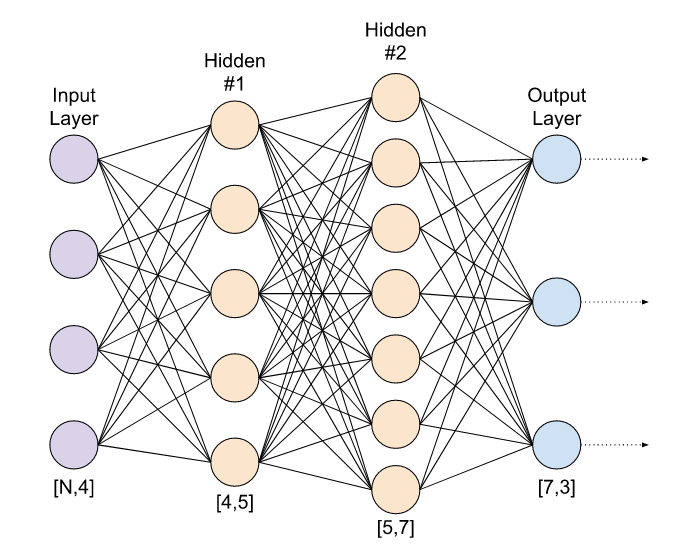
\includegraphics[scale=0.4]{ffnn}
\end{figure}
\begin{defn}
  A \textbf{feed-forward}, \textbf{deep feed-forward}, or \textbf{multi-layer perceptron} (MLP) network is a collection of layers chained together:
  \[
    y = h_3 (h_2 (h_1 (x))) 
  \]
  The output of one is the input to the next, where each layer is $h_i$.
\end{defn}

\begin{itemize}
  \item \textbf{Depth} - number of layers.
  \item \textbf{Width} - number of neurons.
  \item \textbf{Architecture} - how many units the layers have, how the units are connected, etc.
  \item \textbf{Hidden layers} - the layers between the input and output; they do not interact with the outside world.
\end{itemize}
The input layer is conceptual as it computes no transformation, $x = f(x)$.

More formally:
\[
  A^{(l)}  = f^{(l)} (Z^{(l)}); Z^{(l)} = W^{(l)} \cdot A^{(l - 1)}; A^{(0)} = x
\]
where $A^{(l)}$ is the input to the next layer, and $Z$ is referred to as the pre-activation output.

\subsubsection{Initializing Weights}
Two basic ways of initializing the weights of the network are:
\begin{itemize}
  \item \textbf{Zeros} - set parameters to $0$, commonly used for bias.
  \item \textbf{Normal} - set parameters from a normal distribution $W \sim \mathcal{N}(0, 1)$.
\end{itemize}

However, assigning random values could result in tiny or massive outputs - we want the variance of the output of the layers to stay stable across the layers.
\begin{defn}
  The \textbf{Xavier uniform} or \textbf{Glorot uniform} is:
  \[
    W \sim U \left[ -\frac{\sqrt{6}}{\sqrt{n_j + n_{j + 1}}}, \frac{\sqrt{6}}{\sqrt{n_j + n_{j + 1}}}\right] 
  \]
  where $U$ is the uniform distribution, $n_j$ is the number of inputs of the layer, $n_{j + 1}$ is the number of outputs of the layer.
\end{defn}

\section{Activation Functions}
\begin{figure}[htb!]
  \centering
  \caption{Common activation functions.}
  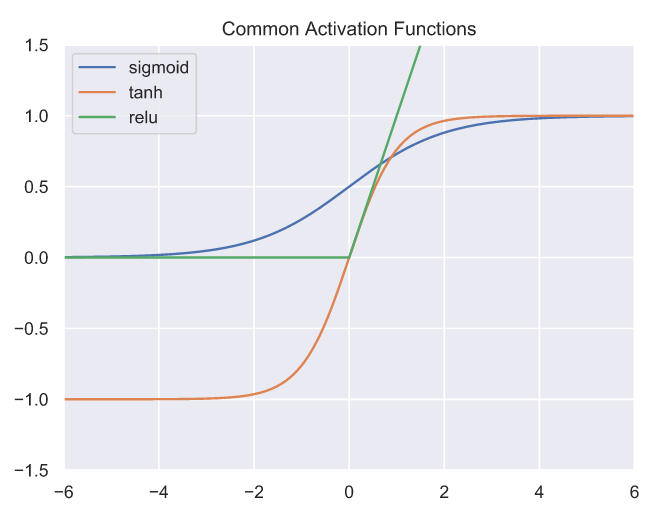
\includegraphics[scale=0.4]{caf}
\end{figure}
The \textit{threshold function} is a linear activation function.
To learn beyond this, we need non-linear activation functions, the most common of which are:
\begin{itemize}
  \item \textbf{linear (identity)} - same as no activation function, simply exposes the linear transformation that precedes the activation $y = W^\intercal x$.
  \item \textbf{sigmoid} - compresses the output to $[0, 1]$, with $0$ corresponding to $0.5$.
    \[
      \text{sigmoid}(x) = \frac{1}{1 + (e^{-x})} 
    \]
  \item \textbf{tanh} - adjusts the sigmoid such that input $0$ corresponds to output $0$, so ranges $[-1, 1]$.
    \[
      \text{tanh}(x) = \frac{2}{1 + (e^{-2x})} - 1 
    \]
  \item \textbf{ReLU} (rectified linear unit) - most commonly used for feed-forward neural networks; piece-wise linear function as it is composed of linear functions but overall it is a non-linear function.
    \[
      \text{relu}(x) =
      \begin{cases}
        x, & \text{if } x > 0 \\
        0, & \text{otherwise}
      \end{cases}
    \]
  \item \textbf{softmax} - $n$-dimensional version of sigmoid; compresses the sum of the output vector to $1$.
    \[
      \text{softmax}(z_i) = \frac{e^{z_i}}{\sum_k e^{z_k}}; z \in \mathcal{R}^n 
    \]
\end{itemize}

We often use ReLU in the hidden layers to get the computational benefits and stability of linear functions, while having non-linearity.
The final layer activation depends on what we are trying to achieve with the network: binary classification, multi-class, or regression? 

\section{Loss Functions}
\begin{defn}
  The \textbf{loss function} is the function we are trying to minimize, such that we learn the relationship between the given inputs and the desired outputs.
\end{defn}

It is crucial to select/design the function in order to learn something meaningful - it depends on what we are trying to do.

\subsection{Regression}
When trying to predict a continuous variable, we have a (non-linear) \textbf{regression problem}.

We use the \textbf{squared error} loss function:
\[
  L(y^{(i)}, a^{(i)})  = (a^{(i)} - y^{(i)})^2
\]
where $a^{(i)}$ is the network output and $y^{(i)}$ the desired output.

When there are multiple outputs, we take the \textbf{mean-squared error}:
\[
  \frac{1}{d} \sum_j^d (a_j^{(i)} - y_j^{(i)})^2 
\]

For the activation of the last layer, since the output is not bounded we use linear activation when regressing with the squared error loss function.

\subsection{Classification}
More commonly, we are trying to classify things categorically.
\textbf{Binary classification} refers to a situation with two classes, \textbf{multi-class classification} with many classes.
We assume every input belongs to one class, and one class only - if we want to predict multiple classes, we need \textbf{multi-label classification}.

\begin{center}
  \begin{tabular}{c | c | c | c}
    Type & Layer Activation & Desired Output & Loss \\
    \hline
    binary & sigmoid & 0 or 1 & binary cross entropy \\
    multi-class & softmax & one-hot & categorical cross entropy \\
    multi-label & sigmoid & 0s and 1s & binary cross entropy
  \end{tabular}
\end{center}

Consider first the sigmoid activation, where values range from $0$ to $1$.
We can interpret this as the probability of that input belonging to a class, $p(y \mid x)$.
The network output is the probability distribution over classes, so we would like to maximize the likelihood of the network assigning the correct labels to all inputs in the dataset:
\[
  \prod_i^N p(y^{(i)} \mid x^{(i)}; \theta) 
\]
assuming that the examples are independent and identically distributed (i.i.d).
For a \textbf{binary classification}, we get:
\[
  \prod_i^N (a^{(i)})^{y^{(i)}} (1 - a^{(i)})^{1 - y^{(i)}}
\]
If we output the same label as the desired label, we get $1$, if we output the opposite we get $0$.
We want to maximize towards $1$, we take the logarithm:
\[
  \sum_i^N y^{(i)}\log(a^{(i)}) + (1 - y^{(i)}) \log(1 - a^{(i)})
\]
since maximizing the logarithm is the same as maximizing the original product.
We then take the inner equation defined on a single pair:
\[
  L(y^{(i)}, a^{(i)}) = -(y^{(i)}\log(a^{(i)}) + (1 - y^{(i)}) \log(1 - a^{(i)}))
\]
which is the \textbf{binary cross entropy} loss function, also referred to as \textbf{negative log likelihood}.
When optimizing, we want to minimize the loss - minimizing the minus of the original equation maximizes the quantity we are interested in.

Extending to the \textbf{multi-class situation}:
\[
  L(y^{(i)}, a^{(i)}) = -\sum_k y_k^{(i)}\log(a_k^{(i)})
\]
is the \textbf{categorical cross entropy} loss function, where $k$ is the number of classes we have.
We use the softmax activation function in the final layer, to get $a^{(i)}$ which yields a probability distribution, e.g.\ $[0.2, 0.6, 0.2]$ with desired output $[0, 1, 0]$.

We could still use squared error with sigmoid activation, but using log-based-loss provides \textbf{better convergence} properties.

\section{Training}
Our network still has random weights, we need to adjust these to fit the desired data - \textbf{training}.

\subsection{Back Propagation}
Let us take the partial derivative of the loss function with respect to the weights of a layer, using the chain rule:
\[
  \frac{\partial Loss}{\partial W^{(L)}} = \frac{\partial Loss}{\partial A^{(L)}} \cdot \frac{\partial A^{(L)}}{\partial Z^{(L)}} \cdot \frac{\partial Z^{(L)}}{\partial W^{(L)}}
\]
We are taking the partial derivative of the loss with respect to every weight in the layer because we want to adjust all of them.

Let us look at the hidden layer before the output layer:
\[
  \frac{\partial Loss}{\partial W^{(L - 1)}} = \frac{\partial Loss}{\partial A^{(L)}} \cdot \frac{\partial A^{(L)}}{\partial Z^{(L)}} \cdot \frac{\partial Z^{(L)}}{\partial A^{(L - 1)}} \cdot \frac{\partial A^{(L - 1)}}{\partial Z^{(L - 1)}} \cdot \frac{\partial Z^{(L - 1)}}{\partial W^{(L - 1)}}
\]
Observe the pattern, we are following the forward computation backwards, starting at the output and going backwards to the weights - \textbf{back-propagation}.
We propagate the gradients backwards through the network layers.
If we extract the pattern out, it reads:
\[
  \frac{\partial Loss}{\partial W^{(L)}}  = \text{ gradient w.r.t. my output } \times \text{ gradient w.r.t. my weights}
\]

\begin{figure}[htb!]
  \centering
  \caption{Back-propagation of gradients of a linear layer.}
  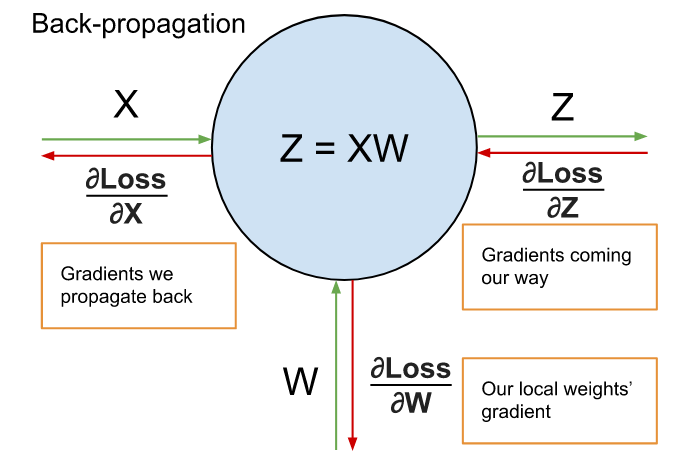
\includegraphics[scale=0.4]{backpropagation}
\end{figure}

When we change the value of $W^{(L - 1)}$, this affects $Z^{(L - 1)}$, which affects $A^{(L - 1)}$, which is the input to the next layer, so this affects $Z^{(L)}$, and so on.

We now consider a linear layer $Z = XW + B$, where:
  \begin{itemize}
    \item $X \in \mathcal{R}^{N \times D}$; consider $N$ as the number of elements in the input, each with $D$ features.
    \item $W \in \mathcal{R}^{D \times M}$; $M$ is the number of outputs for each of our inputs.
    \item $B \in \mathcal{R}^{N \times M}$; this is the stacked version of $b \in \mathcal{R}^{1 \times M}$.
  \end{itemize}
such that $Z \in \mathcal{R}^{N  \times M}$.

\subsection{Back Propagation Example}
Let $N = D = 2$, and $M = 3$:
\[
  X = 
  \begin{bmatrix}
    x_{1, 1} & x_{1, 2} \\
    x_{2, 1} & x_{2, 2}
  \end{bmatrix}
\]
\[
  W =
  \begin{bmatrix}
    w_{1, 1} & w_{1, 2} & w_{1, 3} \\
    w_{2, 1} & w_{2, 2} & w_{2, 3}
  \end{bmatrix}
\]
\[
  B = \begin{bmatrix} \textbf{b} \\ \textbf{b} \end{bmatrix} 
  = \begin{bmatrix}
    b_1 & b_2 & b_3 \\
    b_1 & b_2 & b_3
  \end{bmatrix}
\]
\[
  Z = \begin{bmatrix}
    x_{1,1}w_{1,1} + x_{1,2}w_{2,1} + b_1 & 
    x_{1,1}w_{1,2} + x_{1,2}w_{2,2} + b_2 &
    x_{1,1}w_{1,3} + x_{1,2}w_{2,3} + b_3 \\
    x_{2,1}w_{1,1} + x_{2,2}w_{2,1} + b_1 & 
    x_{2,1}w_{1,2} + x_{2,2}w_{2,2} + b_2 &
    x_{2,1}w_{1,3} + x_{2,2}w_{2,3} + b_3
  \end{bmatrix}
\]
The $Z$ is used in the upper layers, which then pass back a gradient for each of our outputs:
\[
  \frac{\partial Loss}{\partial Z} = \begin{bmatrix}
    \frac{\partial Loss}{\partial z_{1, 1}} &
    \frac{\partial Loss}{\partial z_{1, 2}} &
    \frac{\partial Loss}{\partial z_{1, 3}} \\
    \frac{\partial Loss}{\partial z_{2, 1}} &
    \frac{\partial Loss}{\partial z_{2, 2}} &
    \frac{\partial Loss}{\partial z_{2, 3}}
  \end{bmatrix}
\]
We are interested in the gradients with respect to $W$, $b$, and $X$:
\begin{itemize}
  \item We use $\frac{\partial Loss}{\partial W}$ and $\frac{\partial Loss}{\partial b}$ to \textbf{learn}:
    \begin{align*}
      \frac{\partial Loss}{\partial W} &= \frac{\partial Loss}{\partial Z} \cdot \frac{\partial Z}{\partial W} \\
      \frac{\partial Loss}{\partial b} &= \frac{\partial Loss}{\partial Z} \cdot \frac{\partial Z}{\partial b}
    \end{align*}
  \item We pass $\frac{\partial Loss}{\partial X}$ \textbf{backwards}:
    \[
      \frac{\partial Loss}{\partial X} = \frac{\partial Loss}{\partial Z} \cdot \frac{\partial Z}{\partial X}
    \]
\end{itemize}

Let us take one element and investigate.
We first apply the derivative:
\[
  \frac{\partial Z}{\partial x_{1, 1}} = \begin{bmatrix}
    w_{1, 1} & w_{1, 2} & w_{1, 3} \\
    0 & 0 & 0
  \end{bmatrix}
\]
Then the chain rule:
\[
  \frac{\partial Loss}{\partial x_{1, 1}} = \begin{bmatrix}
    \frac{\partial Loss}{\partial z_{1, 1}} &
    \frac{\partial Loss}{\partial z_{1, 2}} &
    \frac{\partial Loss}{\partial z_{1, 3}} \\
    \frac{\partial Loss}{\partial z_{2, 1}} &
    \frac{\partial Loss}{\partial z_{2, 2}} &
    \frac{\partial Loss}{\partial z_{2, 3}}
  \end{bmatrix}
  \cdot
  \begin{bmatrix}
    w_{1, 1} & w_{1, 2} & w_{1, 3} \\
    0 & 0 & 0
  \end{bmatrix}
\]
Which is the general dot-product:
\[
  \frac{\partial Loss}{\partial x_{1, 1}} = 
  \frac{\partial Loss}{\partial z_{1,1}}w_{1,1} +
  \frac{\partial Loss}{\partial z_{1,2}}w_{1,2} +
  \frac{\partial Loss}{\partial z_{1,3}}w_{1,3}
\]
If we apply this to every element of $X$, we get:
\[
  \frac{\partial Loss}{\partial X} =
  \begin{bmatrix}
  \frac{\partial Loss}{\partial z_{1,1}}w_{1,1} + \frac{\partial Loss}{\partial z_{1,2}}w_{1,2} + \frac{\partial Loss}{\partial z_{1,3}}w_{1,3}
  &
  \frac{\partial Loss}{\partial z_{1,1}}w_{2,1} + \frac{\partial Loss}{\partial z_{1,2}}w_{2,2} + \frac{\partial Loss}{\partial z_{1,3}}w_{2,3} \\
  \frac{\partial Loss}{\partial z_{2,1}}w_{1,1} + \frac{\partial Loss}{\partial z_{2,2}}w_{1,2} + \frac{\partial Loss}{\partial z_{2,3}}w_{1,3}
  &
  \frac{\partial Loss}{\partial z_{2,1}}w_{2,1} + \frac{\partial Loss}{\partial z_{2,2}}w_{2,2} + \frac{\partial Loss}{\partial z_{2,3}}w_{2,3}
  \end{bmatrix}
\]
Which is the same as:
\[
  \frac{\partial Loss}{\partial X} = \frac{\partial Loss}{\partial Z}W^\intercal 
\]

In a similar fashion, we can obtain:
\[
  \frac{\partial Loss}{\partial W} = X^\intercal\frac{\partial Loss}{\partial Z}
\]
\[
  \frac{\partial Loss}{\partial b} = \textbf{1}^\intercal\frac{\partial Loss}{\partial Z}
\]

Let us now consider activation functions.
Suppose we have $Z = f(X)$, where $X \in \mathcal{R}^{N \times D}$, and $Z \in \mathcal{R}^{N \times D}$:
\[
  Z = f(X) = \begin{bmatrix} f(x_{1, 1}) & f(x_{1, 2}) \\  f(x_{2, 1}) & f(x_{2, 2})\end{bmatrix}
\]
If we apply the chain rule for a single element:
\[
 \frac{\partial Loss}{\partial x_{1,1}} =
  \begin{bmatrix}
  \frac{\partial Loss}{\partial z_{1,1}} & \frac{\partial Loss}{\partial z_{1,2}} \\
  \frac{\partial Loss}{\partial z_{2,1}} & \frac{\partial Loss}{\partial z_{2,2}}
  \end{bmatrix} \cdot
  \begin{bmatrix}
  f'(x_{1,1}) & 0 \\
  0 & 0
  \end{bmatrix}
  = \frac{\partial Loss}{\partial z_{1,1}} f'(x_{1,1}) 
\]
Generalising, we get:
\begin{align*}
  \frac{\partial Loss}{\partial X} &=
  \begin{bmatrix}
  \frac{\partial Loss}{\partial z_{1,1}} f'(x_{1,1}) & \frac{\partial Loss}{\partial z_{1,2}} f'(x_{1,2}) \\
  \frac{\partial Loss}{\partial z_{2,1}} f'(x_{2,1}) & \frac{\partial Loss}{\partial z_{2,2}} f'(x_{2,2})
  \end{bmatrix}
  \\
  &=
  \begin{bmatrix}
  \frac{\partial Loss}{\partial z_{1,1}} & \frac{\partial Loss}{\partial z_{1,2}} \\
  \frac{\partial Loss}{\partial z_{2,1}} & \frac{\partial Loss}{\partial z_{2,2}}
  \end{bmatrix} \circ
  \begin{bmatrix}
  f'(x_{1,1}) & f'(x_{1,2}) \\
  f'(x_{2,1}) & f'(x_{2,2})
  \end{bmatrix}
  \\
  &=
  \frac{\partial Loss}{\partial Z} \circ f'(X)
\end{align*}
where $\circ$ is element-wise multiplication (\textit{Hadamard product}).

The derivatives for some of the activation functions are:
\begin{itemize}
  \item \textbf{linear}: $f'(x) = 1$, for all $x$.
  \item \textbf{sigmoid (logistic)}: $f'(x) = f(x)(1-f(x))$.
  \item \textbf{tanh}: $f'(x) = 1-f^2(x)$.
  \item \textbf{ReLU}: $f'(x) = 1$, if $x > 0$.
\end{itemize}
Notice that for sigmoid and tanh, the gradients range $[0, 1]$, then as you back propagate, the gradients can vanish - \textbf{vanishing gradient problem}.
This is not the case with ReLU.

\section{Gradient Descent}
Once we have the direction we want to adjust the weights to, we iteratively descend in the direction of the gradient to slowly minimize the loss - \textbf{gradient descent}:
\begin{enumerate}
  \item Start with random weights/parameters $\theta$.
  \item Compute the gradients with respect to some data and loss function, also called an \textbf{objective function} $J(\theta)$.
  \item Adjust weights in the direction of the gradient.
  \item Repeat until we reach some minimum.
\end{enumerate}
A non-linear function can have multiple \textbf{local minimum}, there is no guarantee we will converge to the \textbf{global maximum}.

\[
  W \leftarrow W - \alpha \frac{\partial L}{\partial W} 
\]
where $\alpha$ is the \textbf{learning rate}, how much of a leap we should take in that direction.

In order to use this, we assume that the gradient can be computed for every parameter - we need our functions, network, and loss to be differentiable.

\subsection{Batches}
Ideally we would like to compute the gradient using the entire training data but this is expensive and slow.
Instead we estimate the true gradient using \textbf{small random batches}:
\begin{itemize}
  \item \textbf{Stochastic Gradient Descent (SGD)} - take one random data point and immediately update the weights using that gradient.
  \item \textbf{Batch Gradient Descent} - use the entire data set then update the weights.
  \item \textbf{Mini-batch Gradient Descent} - take small batches at a time then update the weights.
\end{itemize}

In mini-batch gradient descent:
\begin{enumerate}
  \item Take training data $X \in \mathcal{R}^{N \times D}$, size $N$ each with $D$ features.
  \item Shuffle $X$ so that the points are not grouped together - helps with convergence due to the different combinations of data points.
  \item Chop into batches of size $B$, such that they have the shape $B \times D$.
  \item Compute the forward pass to collect the network output with one batch.
  \item Compute the derivative of the loss with respect to the network outputs.
  \item Back-propagate the gradients to compute the derivative loss with respect to every parameter in the network.
  \item Update the weights using the given learning rate $\alpha$.
  \item Repeat for every batch.
  \item After we have done this for every batch we have finished an \textbf{epoch}, we then repeat on the batches until we have done the required number of epochs or reached a convergence criteria.
\end{enumerate}

\subsection{Hyper-Parameters}
Anything not learned, e.g.\ number of layers, units in each layer, learning rate, are set by the user - \textbf{hyper-parameter}.
Finding, guessing, and tuning is required to find the best values.

\subsection{Learning Rate Decay}
We can extend gradient descent to be adaptive by performing \textbf{learning rate decay}:
\[
  \alpha \leftarrow \alpha d 
\]
where $d \in [0, 1]$, which reduces the learning rate by a factor each epoch.

As we approach the minimal loss, we would like to take smaller steps to avoid overshooting.

\section{Neural Network Evaluation}
Validation data is used to tune the hyper-parameters of the model.
We then use the best model on the validation set as our final model, and test on the test data.

To split the data into sets, we can use k-fold cross validation or just a simple split.

\subsection{Overfitting}
Noise can be present in the data, we want to avoid our model overfitting to a data set so that it does not learn from noisy data.

We can detect overfitting by looking at the loss value or accuracy over time with respect to the training and validation data.
Initially training and validation loss will decrease as the network learns, but at some point the \textbf{validation loss will start to increase while training loss continues to decrease} - overfitting has started.

To avoid this, we can do \textbf{early stopping} to stop the training when validation loss starts to stray from the training loss.

There is a correlation between network capacity (the number of layers, and the number of units those layers have) and overfitting:
\begin{itemize}
  \item If the network is underfitting then it may not have enough capacity, we can try increasing the number of units/layers.
  \item If the network is overfitting then it may have too much capacity, we can try decreasing the number of units/layers.
\end{itemize}

The best solution to overfitting is getting more data - there is less opportunity for the network to memorize specifics about the training set as there are more training points.

\subsection{Regularisation}
If our data has complex patterns we want to introduce more capacity, but this has the tendency to overfit.
\textbf{Regularisation} is a way to penalise the model to stop it from overfitting - we reduce the effective capacity of the network by penalising how large the weights could be.

If a feature is present that describes only the training data, the network may latch onto it and aggressively try to learn it, we can penalise this by:
\begin{itemize}
  \item \textbf{L2 Regularisation}
    \begin{align*}
      J(\theta) = Loss(Y, A) + \lambda \sum_w w^2 &&
      w \leftarrow w - \alpha \left( \frac{\partial Loss}{\partial w} + 2 \lambda w \right)
    \end{align*}
    \begin{itemize}
      \item As the weight increases, so does loss due to $w^2$ - to reduce loss the network must keep $w$ small.
      \item $\lambda$ tells us how much we want to regularize.
      \item The weight update rule is proportional to weight - larger weights shrink proportionally faster.
    \end{itemize}
  \item \textbf{L2 Regularisation}
    \begin{align*}
      J(\theta) = Loss(Y, A) + \lambda \sum_w \lvert w \rvert &&
      w \leftarrow w - \alpha \left( \frac{\partial Loss}{\partial w} + \lambda \text{sign}(w) \right)
    \end{align*}
    \begin{itemize}
      \item The absolute value of the weight is added to the objective function.
      \item The update rule considers a fixed movement towards 0 - if it is negative it is nudged upwards, if positive it is nudged downwards by a fixed $\lambda$ amount.
    \end{itemize}
\end{itemize}
These may also be referred to as \textbf{weight decay} as they both decay weights to 0.
This results in less capacity as a weight of 0 implies no connection, we are simplifying the network by removing its ability to learn very specific patterns of the training set. \\

L1 produces sparse weights as weights are pushed to 0, only the most useful features will have non-zero weight - feature selection.

L2 ensures smoothness as it encourages a combination of inputs/features to be used, since weights are not forced to 0 when they are already small.
A large combination of features are used over a few.

We can mix these so in the final layer we may want to pick certain features and use L1, whereas we could use L2 in the hidden layers.

\subsubsection{Dropout}
When we push the weights towards 0, the connection is effectively cut and capacity reduced.
We could remove them entirely and not have fully-connected layers - \textbf{dropout}.
The outputs of layers are randomly set to 0, essentially turning off neurons.

During each round, we set the output of the neuron to 0 with probability $p$.
Every time we apply dropout we get a different sub-network, so it is like training smaller networks inside a larger one - \textbf{interdependency between neurons across layers is reduced} as neurons may be dropped in the next round.
The network becomes more robust as it is less ability to extract specific features of the training data.

Dropout is \textbf{applied only at training time}, during test or prediction time the entire network is active and no neuron is dropped - but the weights/activations may be scaled to avoid saturating neurons since all connections are active.

Since the network is dissected, we may need more epochs.
As gradients become 0, a higher learning rate would also be helpful.

\subsubsection{Pre-processing}
To better utilise our data, we can apply some pre-processing to remove trivial relationships in the training data which may cause overfitting.

One approach is \textbf{data augmentation} which introduces noise to the data:
\[
  X' = X + \mathcal{N}(\mu, \sigma^2) 
\]
This wiggles specific features/points in the data using Gaussian noise so that they are no longer static - we are generating artifical data based on the original data, giving better generalisation and reducing overfitting.
For example, we could blur and flip images when doing image recognition.

A more common technique is \textbf{data normalisation} where we normalize the input, and potentially the output data.
This may be in the form of \textbf{feature scaling} to reduce a range to $[0, 1]$ or $[-1, 1]$, or normalising using the mean and standard deviation of the data $X' = \frac{X - \mu}{\sigma}$ (\textbf{z-normalisation}).

Recall $\frac{\partial Loss}{\partial W} = X^\intercal \frac{\partial Loss}{\partial Z}$, if $X$ has very large or very small inputs then training is destabilised or hampered.

\section{Unsupervised Learning}
Unsupervised learning is usually done with \textbf{clustering} - grouping data together in the feature space.
\begin{defn}
  A \textbf{cluster} is a collection of data items which are similar between them, and dissimilar to data items in other clusters.
\end{defn}
An unsupervised learning problem is one where the right label does not exist, we want to see if we can cluster the data points to form classes.

\subsection{$k$-Means}
\begin{enumerate}
  \item \textbf{Initialisation}:
    \begin{itemize}
      \item Select the number of clusters $k$.
      \item Randomly place $k$ centroids in the feature space.
    \end{itemize}
  \item \textbf{Assignment}:
    \begin{itemize}
      \item Assign each data point to the nearest centroid.
    \end{itemize}
  \item \textbf{Update}:
    \begin{itemize}
      \item Update the position of each centroid by computing the mean position of all the data points associated to the centroid.
    \end{itemize}
  \item \textbf{Repeat}:
    \begin{itemize}
      \item As the centroid positions have changed, the points must be reassigned and the centroids updated until there is convergence.
    \end{itemize}
\end{enumerate}

\subsection{Selection of $k$}
\subsubsection{Elbow Method}
\begin{figure}[htb!]
  \centering
  \caption{Selecting the elbow point.}
  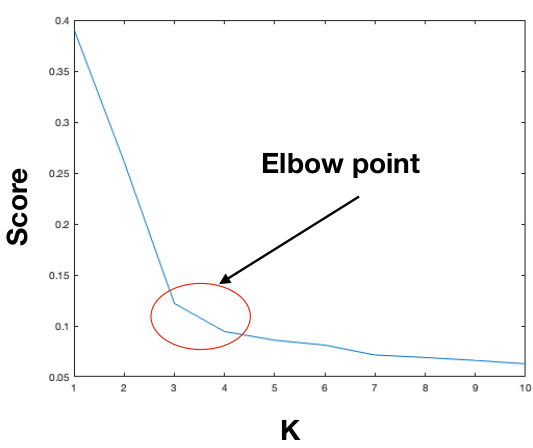
\includegraphics[scale=0.3]{elbow}
\end{figure}
\begin{enumerate}
  \item Run $k$-means forall possible values of $k$.
  \item Compute a score or each - the average of the mean distance to the centroid.
  \item Select the $k$ where the rate of decrease sharply shifts, the \textbf{elbow point}.
\end{enumerate}

\subsubsection{Cross-Validation}
\begin{enumerate}
  \item Split the dataset into $N$ folds.
  \item Use $N - 1$ folds to compute the centroid positions with $k$-means.
  \item Compute the average score on the validation datasets.
  \item Do this for various values of $k$, pick the best configuration - select $k$ such that further increases in the number of clusters leads to only small improvement in the average score.
\end{enumerate}

\subsection{Strengths and Weaknesses}
\begin{itemize}
  \item \textbf{Strengths}:
    \begin{itemize}
      \item Easy to understand and implement.
      \item $O(tkn)$, where $t$ is the number of iterations; since $k$, $t$ are small compared to $n$, it is considered linear.
    \end{itemize}
  \item \textbf{Weaknesses}:
    \begin{itemize}
      \item Only a local optimum is found - usually run several times with random initialization to compensate.
      \item Must define $k$.
      \item Only applicable if the mean is defined.
      \item Sensitive to initialization and outliers.
      \item Not suitable for non hyper-ellipsoidic clusters.
    \end{itemize}
\end{itemize}

\section{Density Estimation}
We use \textbf{density estimation} to perform anomoly or novelty detection.

\subsection{Probability Density Functions (PDFs)}
A PDF models the probability of a sample to be generated in a specific area.

Given a dataset, we can see that some regions are denser than others, and model this with a \textbf{Gaussian distribution}:
\begin{itemize}
  \item \textbf{Univariate}:
    \[
      \mathcal{N}(x \mid \mu, \sigma) = \frac{1}{\sqrt{2 \pi \sigma^2}}\exp^{-\frac{(x - \mu)^2}{2 \sigma^2}} 
    \]
  \item \textbf{Multivariate}:
    \[
      \mathcal{N}(\bm{x} \mid \bm{\mu}, \bm{\Sigma}) = \frac{1}{\sqrt{(2\pi)^D \lvert \Sigma \rvert}}\exp^{-\frac{1}{2} (X - \mu)' \Sigma^{-1}(X - \mu)}
    \]
\end{itemize}

For the univariate:
\begin{align*}
  \mu = \frac{1}{N} \sum_{n = 0}^N x_n && \sigma^2 = \frac{1}{N} \sum_{n=0}^N (x_n - \mu)^2
\end{align*}

For the multivariate:
\begin{align*}
  \bm{\mu} = \frac{1}{N} \sum_{n = 0}^N \bm{x_n} && \bm{\Sigma} = \frac{1}{N} \sum_{n=0}^N (\bm{x_n} - \bm{\mu})(\bm{x_n} - \bm{\mu})'
\end{align*}

\subsection{Quality of the Model}
We compute the \textbf{negative-log-likelihood} on the dataset $\mathcal{X}$:
\[
  \mathcal{L} = - \log p(\bm{\mathcal{X}} \mid \bm{\theta}) = - \log \prod_{n = 1}^N p(\bm{x_n} \mid \theta) = - \sum_{n = 1}^N \log(p(\bm{x_n} \mid \bm{\theta})) 
\]

This is analogous to the concept of loss functions - we search for the parameter values that minimize this quantity:
\[
  \mathcal{L} = \frac{N}{2} \log(2 \pi) + \frac{N}{2} \log(\sigma^2) + \frac{1}{2\sigma^2} \sum_{n = 1}^N (x_n - \mu)^2 
\]

The optimum values are when the derviates are equal to $0$, which gives us:
\begin{align*}
  \mu = \frac{1}{N} \sum_{n = 1}^N x_n && \sigma^2 = \frac{1}{N} \sum_{n = 1}^N (x_n - \mu)^2
\end{align*}

\subsection{Gaussian Mixture Model (GMM)}
\begin{figure}[htb!]
  \centering
  \caption{Gaussian v.s.\ Guassian Mixture Model}
  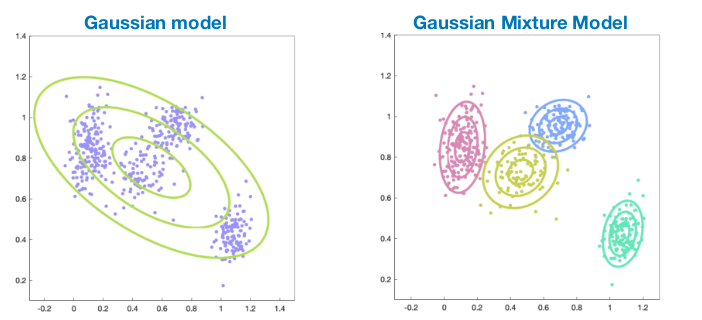
\includegraphics[scale=0.5]{mixture}
\end{figure}
We may need to use a combination of several distributions to construct our model:
\[
  p(\bm{x}) = \sum_{k = 1}^K \pi_k p_k (\bm{x}) 
\]
where $0 \leq \pi_k \leq 1$ and $\sum_{k = 1}^K \pi_k = 1$.

We use the \textbf{Gaussian Mixture Model}:
\[
  p(\bm{x} \mid \theta) = \sum_{k = 1}^K \pi_k \mathcal{N} (\bm{x} \mid \bm{\mu_k}, \bm{\Sigma_k})
\]
where $\bm{\theta} = \{ \bm{\mu_k}, \bm{\Sigma_k}, \bm{\pi_k} : k = 1, \dots, K \}$.

In GMM, all $k$ mixture components contribute to the probability distribute, we can compute the \textbf{responsibility} of the $k$th mixture component for the $n$th data point:
\[
  r_{nk} = \frac{\pi_k \mathcal{N}(\bm{x_n} \mid \bm{\mu_k}, \bm{\Sigma_k})}{\sum_{j = 1}^K \pi_j \mathcal{N} (\bm{x_n} \mid \bm{\mu_j}, \bm{\Sigma_j})
}
\]

\subsubsection{Expectation Maximization (EM)}
We cannot maximise the likelihood to update each parameter, as the update of each parameter depends on the other paramaeters.

Instead we perform \textbf{expectation maximization} on GMM, known as \textbf{GMM-EM}:
\begin{enumerate}
  \item \textbf{Initialization} - for each mixture component, initialize $\bm{\theta}$.
  \item \textbf{E-Step} - compute the responsibilities for each data point and each mixture component.
  \item \textbf{M-Step}:
    \begin{itemize}
      \item Update the mean of each mixture component:
        \[
          \bm{\mu_k} = \frac{1}{N_k} \sum_{n = 1}^N r_{nk} x_n \text{ with } N_k = \sum_{n = 1}^N r_{nk}
        \]
      \item Update the covariance of each mixture component:
        \[
          \bm{\Sigma_k} = \frac{1}{N_k}\sum_{n = 1}^N r_{nk} (\bm{x_n} - \bm{\mu_k})(\bm{x_n} - \bm{\mu_k})' 
        \]
      \item Update the weight of each mixture component:
        \[
          \pi_k = \frac{N_k}{N} 
        \]
    \end{itemize}
  \item Repeat E and M steps until convergence.
\end{enumerate}

We determine convergence through:
\begin{itemize}
  \item No significant variation of the parameters, or
  \item Stagnation of the likelihood.
\end{itemize}
As we may converge to a local optimal, we need to restart the algorithm with different initial guess of parameters.

\subsubsection{Selecting the Number of Components}
\begin{itemize}
  \item More mixture components will lead to higher likelihood but may not generalize well on new data.
  \item \textbf{Cross-validation}.
  \item \textbf{Bayesian Information Criterion} (BIC) - minimize:
    \[
      BIC(K) = \mathcal{L}(K) + \frac{P(K)}{2} \log(N) 
    \]
    where:
    \begin{itemize}
      \item $K$ is the number of mixture components.
      \item $N$ is the number of data points.
      \item $P(K)$ is the number of parameters estimated by the model, e.g.\ for 2D Gaussian $P(K) = 6K$, as 2 for mean, 3 for covariance, 1 for weight.
    \end{itemize}
\end{itemize}

\subsubsection{Relation to $k$-Means}
GMM-EM can be used to do unsupervised classification - each mixture component is a source which generates data points with a different probability.

GMM-EM is like \textbf{soft $k$-means clustering} - every point belongs to several clusters with certain degrees.

\section{Genetic Algorithms}
\begin{defn}
  \textbf{Genetic algorithms} are an optimization algorithm for black-box functions.
  It can be seen as a reinforcement learning problem.
\end{defn}

A common base is:
\begin{enumerate}
  \item Randomly generate a population of solutions.
  \item Each solution is represented by a genotype, which develops into a phenotype (the actual parameters).
  \item A \textbf{fitness function} measures the performance of phenotypes.
  \item The fittest individuals have a higher probability to pass part of their genotype to their offspring.
\end{enumerate}

The differences lie in:
\begin{itemize}
  \item \textbf{Representation of genotype}.
  \item \textbf{Selection operator} - how to select which solutions to reproduce.
  \item \textbf{Cross-over operator} - how to mix the parents' genotypes.
  \item \textbf{Mutation operator} - the type and frequency of variations applied to the genotype after reproduction.
\end{itemize}

\subsection{Fitness Function}
To solve the problem, we maximize fitness - it represents the problem we want to solve.

\subsection{Genotype and Phenotype}
These represent the potential solutions to the problem.
A genotype can be a binary string and the phenotype be the aggregation of this string into trios, and converting each trio into an integer to act as the actual solution.

\subsection{Selection Operator}
This selects the parents of the next generation:
\begin{itemize}
  \item \textbf{Biased roulette wheel} - individuals with a higher fitness have a larger proportion of the roulette circle.
  \item \textbf{Tournament} - randomly draw two individuals and select the best out of the two as the parent, then only relative values of fitness are considered.
\end{itemize}

In general, the new population replaces the old.
With \textbf{elitism}, we may keep a fraction of the best individuals found so far.

\subsection{Cross-over Operator}
Combine the traits of the parents - on a string we can perform \textbf{single-point cross-over}, selecting a random split point and forming two children by exchanging portions of the genotype.

\subsection{Mutation Operator}
To explore nearby solutions, we can randomly choose whether to flip each bit of the string.
We can also add more specific mutation for the problem, e.g.\ swapping groups of bits.

\section{Evolutionary Strategies}
For problems involving real parameters, we use an \textbf{evolutionary strategy}:
\begin{itemize}
  \item \textbf{Genotype} - list of reals.
  \item \textbf{Parent selection} - uniform.
  \item \textbf{Mutation} - Gaussian.
\end{itemize}

\subsection{$(\mu + \lambda)$ - ES}
\begin{enumerate}
  \item Randomly generate a population of size $(\mu + \lambda)$.
  \item Evaluate the population.
  \item Select the $\mu$ best as the parents $x$.
  \item Generate $\lambda$ offspring $y$, from the parents:
    \[
      y_i = x_i + \mathcal{N}(0, \sigma) \text{ where } $j = \text{ random}(\mu)  
    \]
  \item The new population is the union of parents and offspring.
\end{enumerate}

\subsubsection{Finding $\sigma$}
\begin{itemize}
  \item Large $\sigma$ - population moves to solution quickly but hard to refine.
  \item Small $\sigma$ - population moves to solution slowly, more affected by local optimums. 
  \item We can adapt $\sigma$ over time by adding it to the genotype, then:
      \[
        \sigma_i = \sigma_j \exp(\tau_0 \mathcal{N}(0, 1)) 
      \]
      where $\tau_0$ is proportional to $\frac{1}{\sqrt(n)}$.
\end{itemize}


\end{document}
